
Como discutido na introdução, o nexo entre cidadãos e governo é a base dos
sistemas democráticos. Dada a importância desse nexo, não é surpresa que na
Ciência Política exista uma grande gama de trabalhos e abordagens que busquem
descrever, explicar e prever as várias dimensões desse nexo. A caracterização e
justificativa para nosso problema de pesquisa parte de um diálogo com a Teoria
Política Formal, a ser definida e discutida em seguida.

\subsection{Fundamentos da Teoria Política Formal}

Vamos definir Teoria Política Formal como: conjunto de modelos e hipóteses
teóricas explicitamente definidos que buscam representar atividades e
comportamentos relacionados à ação e escolha coletiva.

Com essa definição estamos conjugando três definições: a de Teoria, a de
Política e a de Formal. O conceito de política, e em certa medida o de teoria,
pode ser considerado como ``essencialmente contestado'', isto é, é um conceito
cuja grande importância normativa faz com que haja uma disputa em relação ao seu
uso apropriado \cite{collier2006essentially}. Existe assim ampla literatura
lidando com a melhor definição do que é política. Nós estamos usando a definição
dada por Joe Oppenheimer, para o qual  a ``política consiste
no comportamento realizado com o objetivo de tomar decisões centralizadas para
um grupo, ou para assegurar o interesse de membros desse grupo'' \cite[p.
I]{oppenheimer2012principles}\footnote{Essa definição é equivalente a dada por
  \citeonline{barber2003strong}. Para uma discussão mais aprofundada sobre o
  tema ver: \citeonline{warren1999political}.}.

Quanto a definição de teorias estamos seguindo perspectivas pós-positivistas de
de ciência, particularmente a Visão Semântico-Pragmática de
\citeonline{clarke2012model} em que teorias são conjuntos de modelos, pensados
como representações de sistemas concretos, e hipóteses teóricas - a delimitação
da similaridade dos modelos com determinados sistemas alvo\footnote{Para uma
  discussão sobre as diferentes visões sobre o que são teorias e modelos ver
  \citeonline{sep-structure-scientific-theories}.}.

Por fim, entendemos que os modelos são formais na medida em que construídos por
meio de algum sistema formal \cite{wong2015formal}. Em Teoria Política Formal
isso significa que tendem a ser construídos usando o meio da lógica formal,
matemática ou computação \cite{morton1999methods}. Nosso foco na literatura em
teoria política formal é justificado pelo fato dela ser um corpo teórico
construído por meio de modelos \textit{explícitos} \cite{epstein2008model}, de
forma que a seguinte relação fique clara:

\begin{figure}[H]
  \centering 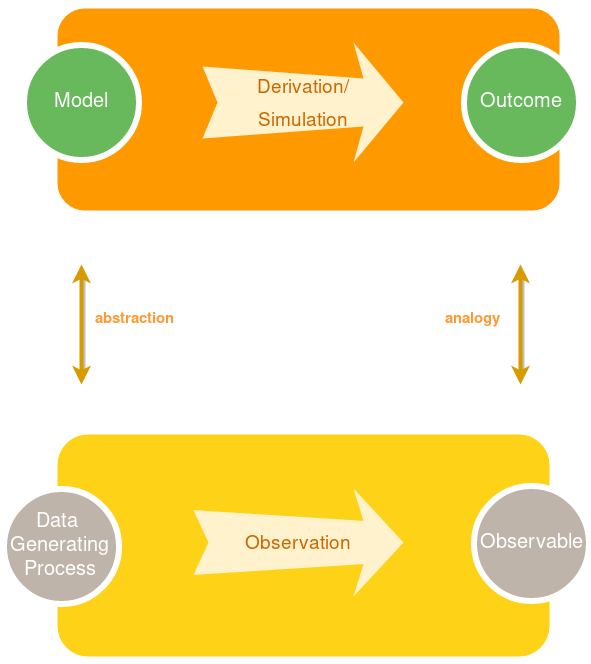
\includegraphics[scale = 0.5]{ims/ms.png}
  \caption{Relação entre Modelos e Sistemas Alvo.}
  Fonte: Adaptado de \citeonline{downey2012think}
\end{figure}










